\documentclass{article}


\usepackage{arxiv}

\usepackage[utf8]{inputenc} % allow utf-8 input
\usepackage[T1]{fontenc}    % use 8-bit T1 fonts
\usepackage{hyperref}       % hyperlinks
\usepackage{url}            % simple URL typesetting
\usepackage{booktabs}       % professional-quality tables
\usepackage{amsfonts}       % blackboard math symbols
\usepackage{nicefrac}       % compact symbols for 1/2, etc.
\usepackage{microtype}      % microtypography
\usepackage{lipsum}
\usepackage{siunitx}
\usepackage{hyperref}
\usepackage[linesnumbered,ruled,vlined]{algorithm2e}
\usepackage{float}
\usepackage{amsmath}
\usepackage{enumerate}
\usepackage{cite}
\usepackage{xcolor}
\usepackage{graphicx}
\graphicspath{ {./img/} }

\newcommand{\note}[1]{\textbf{#1}}

\title{Towards a Customizable Text-to-speech Personal Assistant}


\author{
 Chenyu Shi\\
   s3500063\\
   \And
 Siwen Tu\\
   s3631400\\
   \And
 Shuang Fan \\
   s3505847\\
   \And
 Shupei Li \\
   s3430863\\
}


\begin{document}
\maketitle
\begin{abstract}
The audio assistant technology has been widely applied based on the high development of the deep learning field. In this project, we use deep learning models to accomplish a customizable text-to-speech personal voice assistant. Its main features are twofold --- multi-language support and multi-speaker support. We trained the neural networks on audio datasets and fine-tuned them in different languages with multi-speaker settings. The final model can produce realistic audio based on input texts, and users can customize the type of languages or speaker identities according to their personal preferences.
\end{abstract}


\keywords{VITS \and TTS \and Deep Learning}


\section{Introduction}
\label{sec:intro}

With the rapid development of the deep learning field, text-to-speech techniques are widely applied in our daily lives. For example, they are used in audiobook reading, voice guidance in navigation systems, and human-machine interfaces. One of the most important applications is the voice assistant, such as Siri on the iPhone or Cortana on Windows. These voice assistants can provide help and advice in a speech format, which is more convenient and acceptable than text for humans.

Many languages are spoken worldwide, and people prefer voice assistants to use a familiar language. Additionally, individuals have varying preferences for the type of voice the assistants use, favoring human-like voices over a cold mechanical sound. Hence, customizing voice assistants is a promising direction for this technology.

In this project, we utilize the VITS model \cite{2021kim} to design and implement a customizable text-to-speech personal voice assistant. VITS is a deep learning model for the text-to-speech task based on a conditional variational autoencoder. Our main contributions are as follows. Firstly, we train the VITS model from scratch in Chinese to achieve the multi-language objective since the original VITS implementation was designed for English. In addition, we fine-tune the model based on pre-trained weights in different languages, with a primary focus on Mandarin and Japanese. It further improves the voice assistant's capability --- better output resolution and more language support. Moreover, we fine-tune the model on various types of speakers to complete the goal of multi-speaker. We added five new speakers for Chinese and six for Japanese. The final result is a personal voice assistant that allows users to select their preferred languages and voice types. Through training and evaluation in the experiment, our final model can produce realistic audio based on the input text data, serving as an effective customizable text-to-speech voice assistant.

The rest of the reports will be presented in three sections. In Section \ref{sec:method},  we will show and explain the methodology used in the models. In Section \ref{sec:exper}, the experiment results will be displayed and discussed. And in Section \ref{sec:con}, we will have a conclusion of the report and project.

\section{Methodology}
\label{sec:method}

We describe VITS \cite{2021kim}, the backbone of our TTS assistant, from the perspective of variational inference in detail. We also introduce VITS's architecture and training process to provide a comprehensive overview.

\subsection{CVAEs}
The variational autoencoder (VAE), proposed in \cite{2022kingma}, is a popular approach widely used in unsupervised learning. It is an effective function approximator and can be optimized by the standard stochastic gradient descent (SGD) method. It has shown promising application value in various fields, such as complex pattern recognition, segmentation, future prediction from static images, etc \cite{2021doersch}.

Conditional variational autoencoders (CVAEs) are variants of VAEs. Remember that VAEs learn posterior distribution parameters from dataset $x$ without any label information. In CVAEs, we have additional contextual information $c$ when estimating the posterior distribution. The objective function of the CVAE can be written as follows:
\begin{align}
    \max\quad \log p_{\theta}\left(x|c\right) &- \mathcal{D}\left[q_{\phi} \left(z|x\right)\Vert p_{\theta}\left(z|x \right) \right] 
    \label{eq:objective-function}
\end{align}
where $p_\theta(x|c)$ denotes the marginal log-likelihood of the data, $p_\theta(z|x)$ is the posterior distribution and $q_\phi(z|x)$ is its approximator. According to the definition of Kullback-Leibler divergence and Bayes' theorem, maximizing Equation \ref{eq:objective-function} is equivalent to maximizing the following equation:
\begin{align}
    \max\quad \mathbb{E}_{q_{\phi}(z \mid x)}\left[\log p_{\theta}(x \mid z)-\log \frac{q_{\phi}(z \mid x)}{p_{\theta}(z \mid c)}\right]
    \label{eq:objective-function-equal}
\end{align}
Notice that the relative KL divergence is always a non-negative number. We can derive the evidence lower bound (ELBO) of the objective function based on Equation \ref{eq:objective-function} and Equation \ref{eq:objective-function-equal}:
\begin{align}
    \begin{split}
        \log p_{\theta}(x \mid c) &\geq \mathbb{E}_{q_{\phi}(z \mid x)}\left[\log p_{\theta}(x \mid z)-\log \frac{q_{\phi}(z \mid x)}{p_{\theta}(z \mid c)}\right]\\
                                  &= \underbrace{\mathbb{E}_{q_{\phi}(z|x)}\left[\log p_{\theta}\left(x|z \right)\right]}_{\text{Reconstruction loss}} - \underbrace{\mathcal{D}\left[q_{\phi}(z \mid x) \Vert p_{\theta}(z \mid c) \right]}_{\text{Regularization loss}}
    \end{split}
    \label{eq:elbo}
\end{align}
The ELBO comprises two parts --- the reconstruction loss and the regularization loss. The reconstruction loss describes the data distribution given the latent space, while the regularization loss measures the divergence between the true prior distribution and the encoder's approximate distribution. In practice, we usually choose to minimize the negative ELBO because the term $\mathcal{D}\left[q_{\phi} \left(z|x\right)\Vert p_{\theta}\left(z|x \right) \right]$ is hard to calculate. However, a reasonable posterior approximator $q_\phi(z|x)$ can effectively alleviate the impact of the bias.

\subsection{Expressing VITS as a CVAE}
\begin{figure}[!ht]
    \begin{center}
        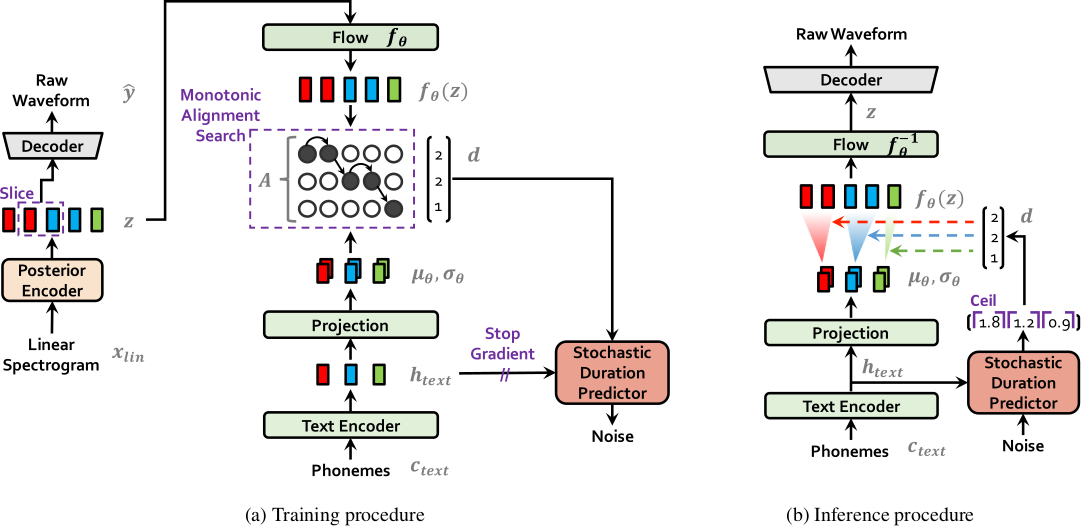
\includegraphics[width=0.95\textwidth]{vits.png}
    \end{center}
    \caption{The architecture of VITS. This figure is directly adapted from \cite{2021kim}.}
    \label{fig:method-vits}
\end{figure}

The architecture of VITS is shown in Figure \ref{fig:method-vits}. VITS model can be expressed as a CVAE. We will illustrate the main idea behind VITS based on the reconstruction loss as well as the regularization loss.

\textbf{Reconstruction Loss}. During the training, we have ground truth soundtracks $x$ and their corresponding text $c_{text}$. Kim et al. \cite{2021kim} define the reconstruction loss as the $L_1$ norm between the input's mel-spectrogram and the estimated mel-spectrogram produced by the model:
\begin{align}
    L_{recon} = \Vert x_{mel} - \hat{x}_{mel} \Vert_1
\end{align}
It is easy to compute the mel-spectrogram $x_{mel}$ of a specific audio file. As for the approximate mel-spectrogram $\hat{x}_{mel}$, we can upsample the latent space to the waveform domain and then transform it to the mel-spectrogram domain.

\textbf{Regularization Loss}. The text-to-speech task requires an automatic alignment between the text input and the corresponding voice features. VITS adopts the monotonic alignment search algorithm to align the audio and textual embeddings. The monotonic alignment search algorithm (MAS) is proposed in \cite{2020kim}. The intuition behind the MAS is applying the dynamic programming algorithm to maximize the likelihood of the data distribution. It will produce an alignment matrix $A$. The condition $c$ in VITS is defined as the concatenation of the text input $c_{text}$ and the alignment matrix $A$, i.e., $c = [c_{text}, A]$. Given the condition $c$, we can calculate the regularization loss following the definition of KL-divergence:
\begin{align}
    \begin{split}
        L_{kl} = \mathcal{D}\left[q_{\phi}(z \mid x) \Vert p_{\theta}(z \mid c) \right]&=\log q_{\phi}\left(z \mid x_{l i n}\right)-\log p_{\theta}\left(z \mid c_{\text {text }}, A\right) \\
        z \sim q_{\phi}\left(z \mid x_{l i n}\right)&=N\left(z ; \mu_{\phi}\left(x_{l i n}\right), \sigma_{\phi}\left(x_{l i n}\right)\right)
    \end{split}
\end{align}
It is worth mentioning that VITS uses the linear-scale spectrogram of the soundtrack $x_{lin}$ instead of the mel-spectrogram. \cite{2021kim} explains that the linear-scale spectrogram is helpful in enhancing the resolution of generated audio. To improve the model's performance further, VITS introduces a normalizing flow $f_\theta$ that connects the conditional prior distribution and the latent space in the following way:
\begin{align}
    p_{\theta}(z \mid c) & =N\left(f_{\theta}(z) ; \mu_{\theta}(c), \sigma_{\theta}(c)\right)\left|\operatorname{det} \frac{\partial f_{\theta}(z)}{\partial z}\right| 
    \label{eq:normalizing-flow}
\end{align}
Equation \ref{eq:normalizing-flow} transforms the latent space into some complex distributions that possess a more powerful expressiveness, which is critical for generating realistic outputs.

\subsection{Training VITS}
The major part of VITS is a CVAE. However, there are more things to consider when handling the text-to-speech task. Firstly, we need to decide the duration of each token in outputs. A straightforward idea is adding a deterministic duration predictor into the model. But this naive method has a big flaw --- it can not reflect the features of different speakers, which limits the model's application in multi-speaker scenarios. Alternatively, VITS designs a stochastic duration preditor whose loss function is $L_{dur}$ and optimizes it with other modules during training.

VITS also integrates adversarial training into the architecture to guide the optimization direction. With a discriminator $D$ and a decoder $G$, VITS combines two kinds of loss in the adversarial training, namely the least-squares loss and the additional feature-matching loss:
\begin{align}
    \begin{split}
        L_{a d v}(D) & =\mathbb{E}_{(y, z)}\left[(D(y)-1)^{2}+(D(G(z)))^{2}\right] \\
        L_{a d v}(G) & =\mathbb{E}_{z}\left[(D(G(z))-1)^{2}\right] \\
        L_{f m}(G) & =\mathbb{E}_{(y, z)}\left[\sum_{l=1}^{T} \frac{1}{N_{l}}\left\|D^{l}(y)-D^{l}(G(z))\right\|_{1}\right]
    \end{split}
\end{align}

Taken together, we can obtain the final loss for VITS training:
\begin{align}
    L_{v a e}=L_{r e c o n}+L_{k l}+L_{d u r}+L_{a d v}(G)+L_{f m}(G)
\end{align}

During the inference stage, we fix all weights and disgard the posterior encoder because we only have the text input. Final outputs are produced by the decoder $G$.

\section{Experiments}
\label{sec:exper}
The hardware and software we use in the experiment are listed below. Our official project website is \url{https://sd12321sd.github.io/api_project.github.io/}. The code of our project is available on \url{ https://github.com/ShupeiLi/api-final-project/tree/master}.

\textbf{Hardware}:
\begin{itemize}
    \item 1 Titan Xp GPU
\end{itemize}
\textbf{Software}:
\begin{minipage}{0.45\textwidth}
    \begin{itemize}
        \item Cython==0.29.21
        \item librosa==0.8.0
        \item matplotlib==3.3.1
        \item numpy==1.18.5
        \item phonemizer==2.2.1
        \item scipy==1.5.2
        \item tensorboard==2.3.0
    \end{itemize}
\end{minipage}
\hfill
\begin{minipage}{0.45\textwidth}
    \begin{itemize}
        \item torch==1.6.0
        \item torchvision==0.7.0
        \item Unidecode==1.1.1
    \item chardet
    \item pypinyin
    \item monotonic\_align
    \item protobuf==3.20.0
    \end{itemize}
\end{minipage}

\subsection{Training from Scratch}\label{sub:train}
To validate the effectiveness of the VITS model, we train the model on the Chinese Standard Mandarin Speech Corpus and record the performance of different training phases.  

\paragraph{Preprocessing}
Due to the distinctive structure of Chinese characters and their relationship with pronunciation, which differs significantly from English, we need to preprocess the raw data containing audio and Chinese text to better align with the training process. We convert Chinese text into representations using the International Phonetic Alphabet (IPA). We establish mappings for Latin to Bopomofo symbols (a phonetic script used in Mandarin Chinese transliteration and writing systems), Bopomofo symbols to Romaji, and Bopomofo symbols to IPA. This involves leveraging external libraries such as \textit{pypinyin}, \textit{jieba}, and \textit{cn2an} to convert Arabic numerals, Latin characters, and Chinese characters into Bopomofo symbols. Additionally, various regular expressions are employed to locate and replace specific elements in the Chinese text. These procedures aim to optimize the data for the training process, facilitating the establishment of a model that captures the relationship between audio and Chinese text.

\paragraph{Experiment Setting}
We train the model for around 96,000 steps, lasting about 48 hours. We record the performance of 0 step, 5,000 steps, 10,000 steps, 30,000 steps, 50,000 steps, 70,000 steps and 96,000 steps to demonstrate a remarkable improvement, which is shown on our project website.

\paragraph{Dataset} Chinese Standard Mandarin Speech\footnote{https://www.data-baker.com/open\_source.html}. This dataset consists of 10,000 sentences which are spoken by a Chinese female who pronounces standard Mandarin. The average length of the sentences is around 16 characters and the audio is recorded at 48kHz 16-bit sampling frequency, in PCM WAV format. The transcribed text of the audio is recorded as a txt file.


\subsection{Fine-tune the Model}
To build a versatile model capable of handling multiple languages and speakers, we perform fine-tuning on the model using separate datasets for Chinese and Japanese speakers. The customized text-to-speech personal assistant, developed through this process, is showcased on our project website.
\paragraph{Preprocessing}
A bit different from the preprocessing of the Chinese dataset, we also built a pipeline for converting the Japanese text to IPA. We build mappings for Romaji to IPA, consonant to their representations. We utilize the \textit{pyopenjtalk} library to convert the Japanese text to Romaji with the accent, and then we deal with some special consonants and convert the Romaji to IPA.

\paragraph{Experiment Setting}
Based on the model trained in Section \ref{sub:train}, we fine-tune the model for around 84,500 steps, which lasts for about 16 hours. We provide five different speakers including child, middle-aged female, middle-aged male, young female and young male speakers for Chinese. Additionally, we include six speakers for the Japanese language, spanning child, young female, young male, middle-aged female, middle-aged male, and aged male voices. The outcomes of this training process are showcased on our project website.

\textbf{Chinese Dataset}: AISHELL-3 for Chinese \cite{AISHELL-3_2020}. This dataset is a large-scale multi-speaker Mandarin speech corpus provided by Beijing Shell Shell Technology Co., Ltd. The corpus contains roughly 88,000 utterances which are spoken by 218 native Chinese Mandarin speakers. These speakers have different genders, ages, and accents which are marked in the corpus.

\textbf{Japanese Dataset}: JVS corpus \cite{takamichi2019jvs}. This dataset consists of Japanese transcripts and multi-speaker audio data. These audio files are recorded by 100 professional speakers who are of different gender and age. The audio is sampled at 24 kHz and the average duration is 10 seconds. For each speaker, they provide 100 different recordings.



\section{Conclusion}
\label{sec:con}
To conclude, we have built a customizable text-to-speech personal audio assistant based on the VITS model and fine-tuned it to achieve optimal performance. Our final model can produce realistic audio based on the content of the input text. Additionally, users can select their preferred languages and types of voices. The model finally works with satisfying performance and efficiency as a personal voice assistant.

For our model, there are several aspects that could potentially be improved in the future. First of all, the number of languages and types of voices in our model is currently limited. However, increasing the supported languages and speakers does not pose significant challenges for the model, considering the existence of the large open-source text-to-speech community. We just need to repeat each step in our experiment with a new audio dataset of a new language or speaker to extend our model. Additionally, the model does not perform equally well on all types of voices and languages in our experiment. To address this issue, we could find and use higher-quality audio datasets for training and fine-tuning the model with increased computing resources.


\bibliographystyle{unsrt}  
\bibliography{references} 

\end{document}
